\documentclass[useAMS,usenatbib]{mn2e}
\usepackage{graphicx}
\usepackage{amssymb}
\usepackage{natbib}
\bibliographystyle{mn2e}
\pdfminorversion=5   % recommended by MNRAS web page


%%% Journal abbreviations.
\def\apj{ApJ}                 % Astrophysical Journal
\def\apjl{ApJL}               % Astrophysical Journal, Letters
\def\apjs{ApJS}               % Astrophysical Journal, Supplement
\def\mnras{MNRAS}             % Monthly Notices of the RAS
\def\aap{A\&A}                % Astronomy and Astrophysics
\def\aaps{A\&AS}              % Astronomy and Astrophysics, Supplement
\def\aj{AJ}                   % Astronomical Journal
\def\physrep{Phys.~Rep.}      % Physics Reports
\def\nat{Nature}              % Nature
\def\araa{ARA\&A}             % Annual Review of Astronomy and Astrophysics
\def\planss{planss}           % Planetary and Space Science
\def\ssr{SSR}                 % Space Science Reviews
\def\sovast{Sov.~Astron.}     % Soviet Astronomy
\def\canjphys{Can. J. Phys.}  % Canadian Journal of physics
\def\nar{New~Astron.}

 
\newcommand{\msun}{{M$_\odot$}}

\topmargin -1cm


\title{Cooling Clouds by Varying Metallicities: Origin of Globular Cluster Bimodality}

\author[R. Fernandez et al.]{Ricardo Fernandez$^{1}$ and Greg L. Bryan$^{1}$\\
$^{1}$Department of Astronomy, Columbia University, 550 West 120th Street, New York, NY 10027, USA}

\begin{document}

\date{}

%\pagerange{\pageref{firstpage}--\pageref{lastpage}} \pubyear{2013}

\maketitle

%\label{firstpage}

\begin{abstract}
Globular Clusters
\end{abstract}

\begin{keywords}
globular clusters - methods:numerical
\end{keywords}

%% ----------------------------------------------------------------
%
\section{Introduction}

Globular clusters (GCs), with typical masses of $10^5$-$10^6$ \msun\ are particularly interesting relics of star formation for a number of reasons: (1) the are very concentrated, with half-mass radii of a few parsecs, indicating that star formation occurred in a particularly dense environment; (2) the stars in a given GC generally have a very narrow spread in ages and metallicity, implying a single stellar population (although recent results have revealed a more nuanced situation here, as we will discuss briefly later), and (3) the metallicity distribution of GCs in external galaxies is generally bimodal (or at least very different from the metallicity distribution of stars in the galaxy as a whole), with a large number of low-metallicity GCs.  Reviews of their properties include Brodie \& Strader (2006), Renzini (2008, 2013), and see also Protegies et al (2010).

This bimodal, or possibly skewed metallicity distribution (e.g. Strader et al. 2003, Peng et. al 2006) is sometimes interpreted as indicating that there are two formation modes: one that produced low-metallicity, old systems and a second for the generally younger, higher-metallicity component.  For instance, Ashman \& Zepf (1992) suggested that metal-rich GCs are formed in gas rich mergers and metal-poor GCs are donated by progenitor spirals.  However, their work did not incorporate a cosmological model, and their predictions of the number and color distribution of GCs in massive Es galaxies were not consistent, as pointed out by Forbes, Brodie \& Grillmair (1997).  Other models explored reionization for setting the bimodality (e.g., Santos 2003; Harris \& Pudritz 1994).

Beasley et al. (2002) augmented this picture by incorporating a semi-analytical model of combined galaxy and GC formation in a cosmological context. In that work, each mode of GC formation was assigned a fixed efficiency relative to the field stars. However, to match observed values, the formation of metal-poor GCs had to be artificially truncated after $z = 5$. Recently, investigations have explored more empirical, hierarchical galaxy formation models in a cosmological setting.   Muratov \& Gnedin (2010) have modeled the formation of GCs using the assembly history from cosmological simulations combined with observed scaling relations. In their model bimodality naturally arises from the rate of galaxy mergers. Early mergers preferentially produce metal-poor GCs and a few late massive mergers can produce a significant number of metal-rich GCs.  However their model produces metal-rich GCs that are too young, which is at odds with observation that some of metal-rich GCs are old as metal-poor GCs. In addition, their model is again semi-analytic and doesn't explicit deal with how star formation proceeds in low-metallicity, high-density gas.

Essentially none of the models discussed above attempt to model the detailed structure of star formation within globular clusters.  In particular, it is not clear how to get a large amount of gas ($10^6$ \msun) into a very small region without star formation occurring during the collapse, which would result in a wide spatial distribution of stars and perhaps even prevent the collapse.  

As an aside, we note that, quite recently, observations have demonstrated that globular clusters are not a single stellar population, but may be composed of multiple generations showing enhanced He and specific abundance changes, particularly those associated with proton-capture processes (e.g., Norris et al 1981; Kraft 1994; Gratton et al. 2001; Carretta et al. 2009).  In addition, photometric data shows a splitting of the man sequence in many GCs (e.g., Piotto 2009; Anderson et al. 2009; Milone et al. 2010).  This has been challenging to explain because, with a few possible exceptions, the Fe abundence distribution is generally very narrow (consistent with observational errors), indicating that supernova self-enrichment plays no role.  A wide range of models have been proposed to explain these abundance irregularities, beginning with the possibility that AGB stars in the 4-8 \msun\ mass range can produce the necessary elements through hot bottom burning (e.g., D'Ercole et al 2010; Ventura et al. 2013).  Other ideas include the existence of Fast Rotating Massive Stars (FRMS; Krause et. al 2013), supermassive stars (Denissenkov \& Hartwick 2014; Denissenkov et. al 2015), and massive interacting binaries (e.g. Mink 2009; Bastian et al. 2013).  All of these solutions are problematic for a number of reasons (e.g. Renzini et al. 2015; Bastian et al. 2015), including the mass budget required to generate the observed number of second generation stars.  However, in this work, we will not explicitly explore this second generation, instead focusing on the problem of understanding star formation in low-metallicity gas.


%% ----------------------------------------------------------------
%
\section{Basic Idea}
\label{sec:basic}

In this paper, we explore a simple idea: can the cooling properties of low-metallicity gas clouds themselves influence how star formation proceeds?  High-metallicity (by which we mean approximately solar metallicity, or even lower -- we will address this point more precisely below) gas cools rapidly, typically on a timescale shorter than the dynamical time, meaning that present day large gas clouds, with masses in the GC range, are typically ``cold", with temperatures well below their virial temperatures and so rapid fragmentation is inevitable.  This generally means that high-metallicity giant molecular clouds will rapidly produce stars before they are completely collapsed and feedback from those stars will result in a low star formation efficiency (REF).  However, for a low enough metallicity, the gas may cool slowly so that the cloud will collapse coherently, not fragmenting until the central gas density is very high.  These high densities promote rapid star formation resulting in high efficiency.  In this way, paradoxically, inefficient cooling may result in more efficiency star formation.

To futher investigate this simple idea we have created one zone models of a cooling parcel of gas. In 
this scenario, the parameter space consits of density, temperature, and metallicity. Once the parameters
are choosen the gas is allowed to cool. The quanity of interest is the ratio of the absolute value of cooling
time to dynamical time $|t_{cool}|/t_{dyn}|$. In our simple one zone model cooling is computed using the
publicily available grackle chemistry library; details of implementation and functionality can be found
in \cite{Bryan2013}.
\begin{figure}
\begin{center}
\mbox{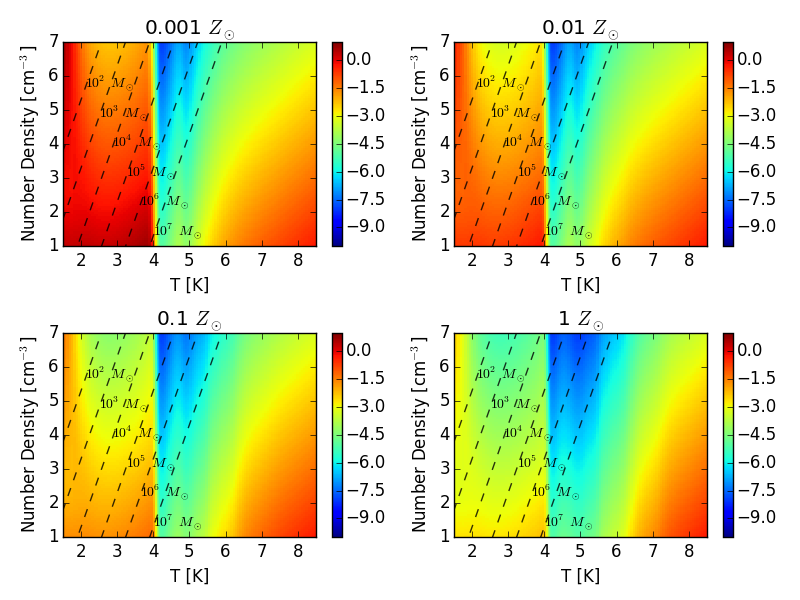
\includegraphics[width=8.5cm]{Images/cooling_to_freefall_no_background}}
\end{center}
\caption{\label{fig:cooling_to_freefall}} Density slice at $t=19.4$ Myr for run with
cooling, turbulence, and metallicity of $Z=10^{-3}Z_\odot$. In this run cooling is
not efficient and gravity takes over forming a dense core. 
\end{figure}

In Figure~\ref{fig:cooling_to_freefall}, is a panel of heat maps of log$(|t_{cool}|/t_{dyn})$
for metallicity values $Z/Z_{\odot}=10^{-3},10^{-2},10^{-1},1$. In the top left corner of Fig~\ref{fig:cooling_to_freefall}
there are two regions where cooling and dynamical time are comparable. The first is in the temperature range of
$10^1-10^4$K, the sharp cutoff at $10^4$K is due to efficient cooling, and the second is in the bottom right
corner. It is the former region that we are most interested because this region is most likely to have
typical values for globular cluster formation. Over each heat map Bonner-Ebert (see ~\ref{sec:numerical} for discription) curves
are overlayed for different mass sizes. It is clear from the plot, for gas clouds of typical mass of globular cluster, ther are 
valuse in the region where cooling is ineffective effectively allowing the gas to collapse coherently. Further, as the metallicity
increases this region becomes less pronounce and the gas becomes more efficent in cooling allowing the gas to cool and fragment
before global collapse sets in.
\begin{figure}
\begin{center}
\mbox{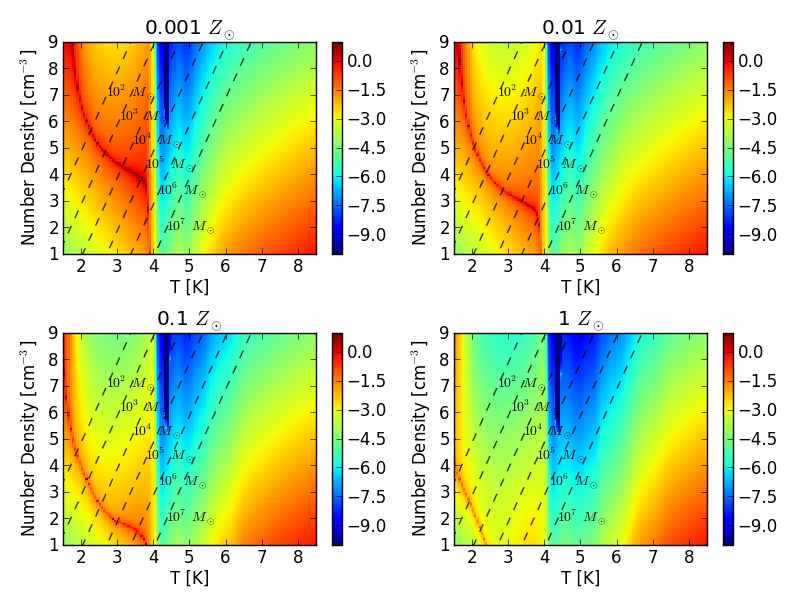
\includegraphics[width=8.5cm]{Images/cooling_to_freefall}}
\end{center}
\caption{\label{fig:cooling_to_freefall_background}} Density slice at $t=19.4$ Myr for run with
cooling, turbulence, and metallicity of $Z=10^{-3}Z_\odot$. In this run cooling is
not efficient and gravity takes over forming a dense core. 
\end{figure}

In Figure ~\ref{fig:cooling_to_freefall_background}, the one zone models are recalculated as previous except allowing
for heating; where heating can be from nearby star fromation. In this situation, an equillibrium curve is present where
heating and cooling are balanced. We no longer have the extended region where cooling and dynamical time scales are 
comparable but know are concentrated along the equillibrium curve. Furthemore, it should be expected that these values should
natuarally seek the equillibrium curve. Therefore, for values above and below the curve there should be a migration
to high density low temperature for values above and low density high temperature for values below. Moreover, when the
the metallicity increase the equilibrium curve shifts downward, decreasing the possibility of having globular cluster
like conditions.

% more...





%% ----------------------------------------------------------------
%
\section{Numerical Models}
\label{sec:numerical}
\subsection{Numerical Method}
This simulations were performed with the publicly available Eulerian three-dimensional
hydrodynamical adaptive mesh refinement Enzo code \citep{Bryan2013}. The domain
box size of the simulation was 150 pc with a top level root grid resolution of $128^3$.
Cell refinement was dictated by baryon mass and Jeans length with a maximum refinement
level of 3. Our simulations included self gravity and radiative cooling using the
Grackle library; details described in \cite{Bryan2013}. The metal heating and
cooling rates are provided from \cite{Haardt2012}.

\subsection{Initial Conditions}
Our initial conditions consisted of a cloud in pressure equilibrium with an
ambient density and temperature background. The internal structure of the
cloud is modeled by a Bonner-Ebert sphere \cite{Bonnor1956}; a self-gravitating
isothermal gas sphere in hydrostatic equilibrium embedded in a pressurized  
medium. To fully describe a Bonner-Ebert sphere, a mass $M_{BE}$, temperature
$T_{BE}$, and an external pressure $P_{ext}$ must be chosen. Following our
assumptions outlined in Section~\ref{sec:basic}, we choosed
$M_{BE}=10^6$ \msun, $T_{BE}=6000$ K, and $P_{ext}=1.8\times10^5\times k_B$
($k_B$ : Boltzmann constant). This corresponds to a cloud on the cusp where
heating and cooling balance. 

In addition, we add turbulence to the cloud following a power spectrum of
$v_k^2 \propto k^{-4}$ for the velocity field.

%% ----------------------------------------------------------------
% 
\section{Results}
\label{sec:results}
\subsection{No Heating Runs}
\begin{figure}
\begin{center}
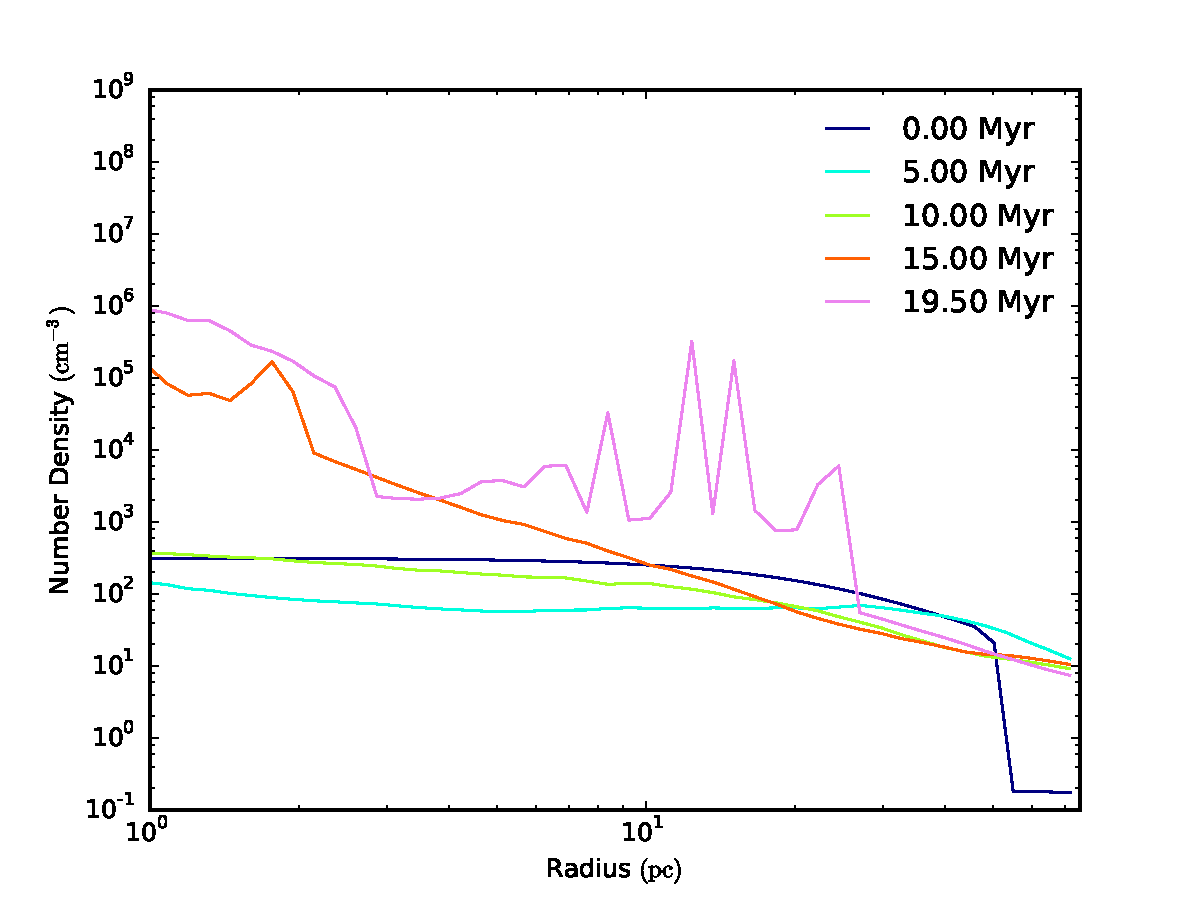
\includegraphics[width=8.5cm]{Images/density_series-eps-converted-to}
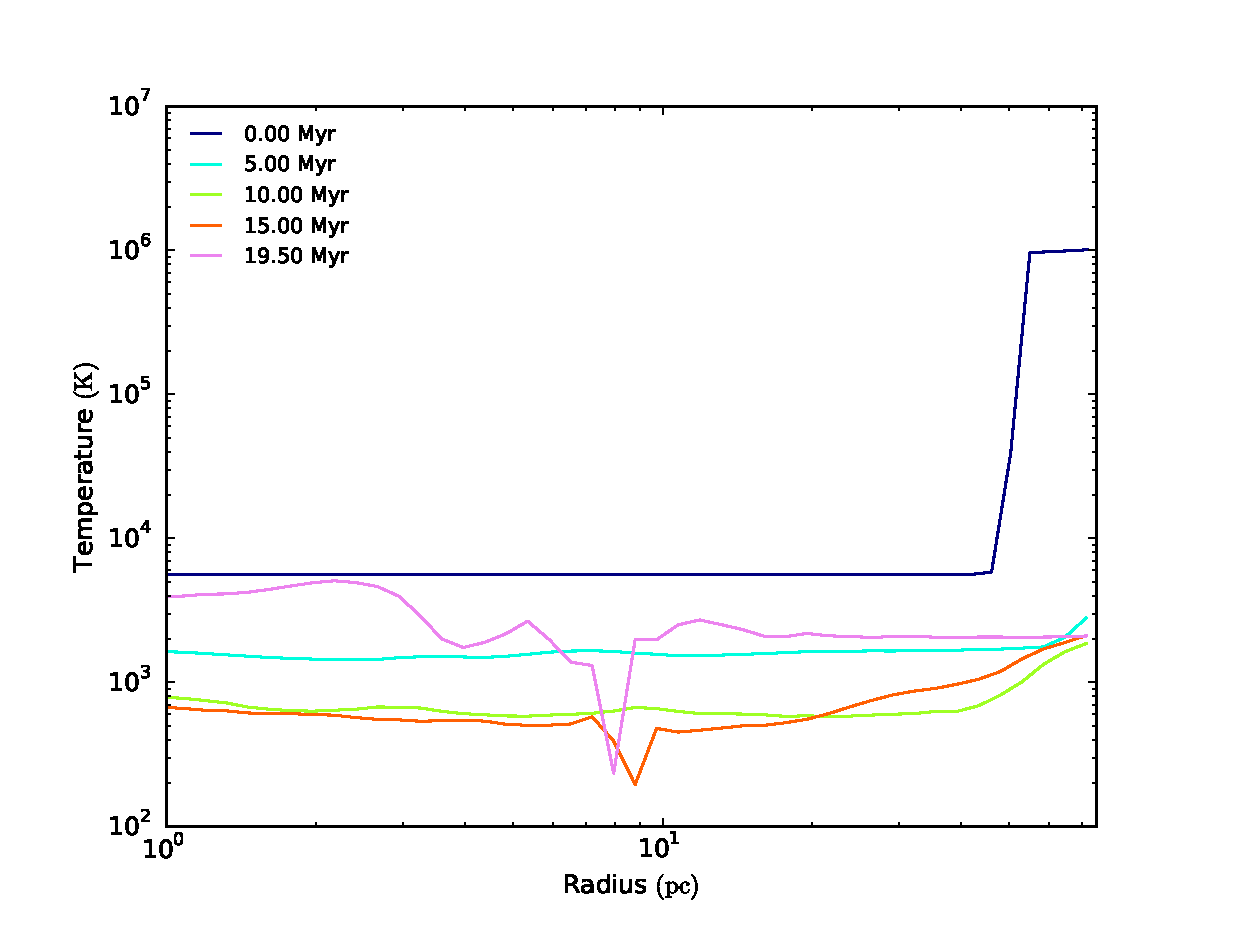
\includegraphics[width=8.5cm]{Images/temperature_series}
\end{center}
\caption{\label{fig:profile_turbulence}} Cell weighted profiles for density
and temperature at give output times for run with cooling, turbulence, and
metallicity of $Z=10^{-3}Z_\odot$.
\end{figure}
In the left hand panel of Figure~\ref{fig:profile_turbulence}, are density profiles at given time steps.
The cloud, which initially stable, starts to change dynamically due the added
turbulence and cooling. The the free fall time of the cloud is $t_{ff}\approx 6$
Myr. However, the added pressure due to turbulence has prolonged any large scale
collapse. Noting the several outputs, the cloud initially starts to drive mass
outward. This is due the increase in pressure from turbulence. The outter rim
of the cloud begins to drive outward decreasing the amount of mass in each radi.
The expansion only last for $\approx 15$ Myr. At this point, gravitational
collapse sets in and the formation of a core begins, see Figure 2. The right
hand panel of Figure~\ref{fig:profile_turbulence}, demonstrates the inability of the cloud to cool
sufficiently. As expected from the one zone model, the cloud cannot efficiently
cool before global gravitational collapse sets in.
\begin{figure}
\begin{center}
\mbox{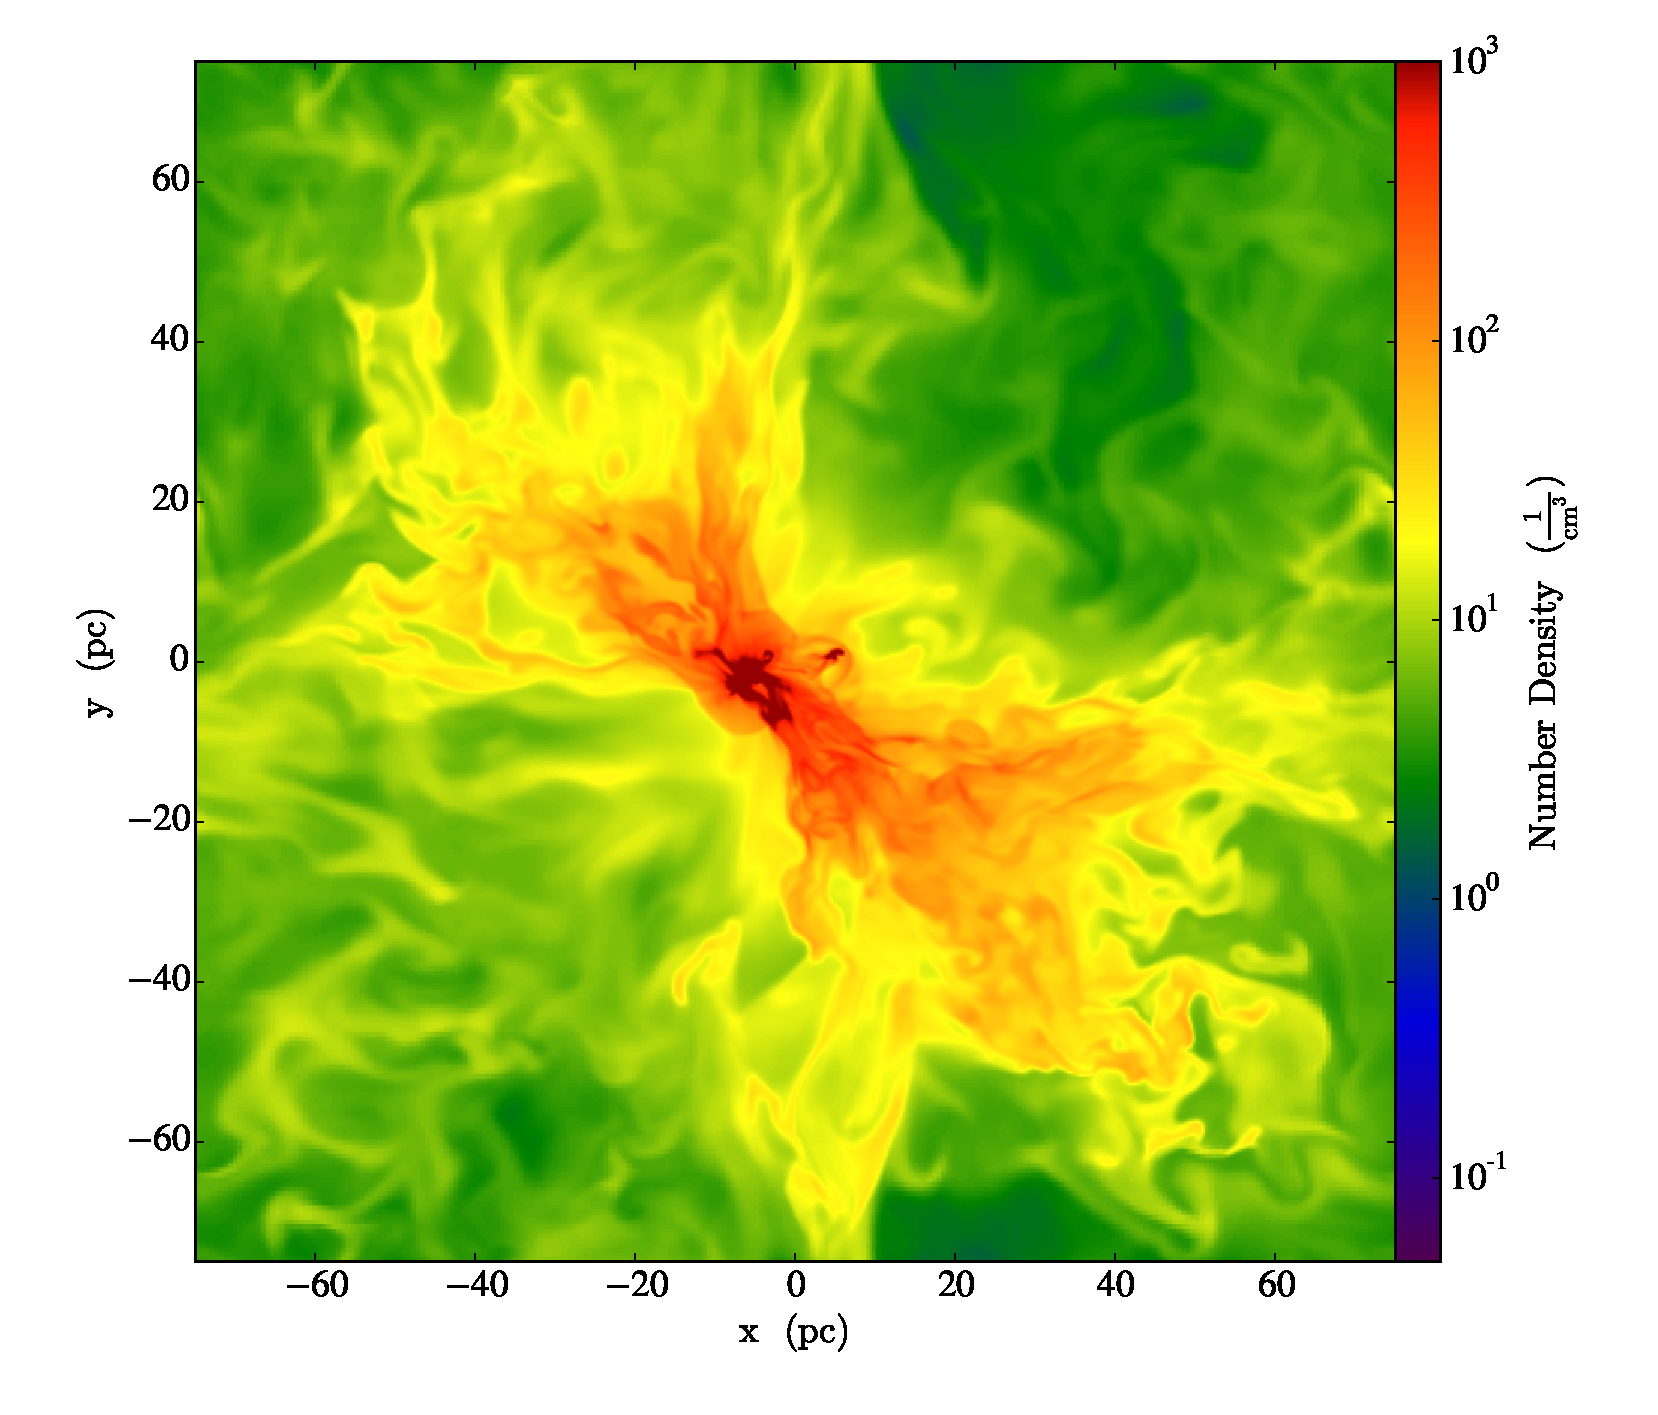
\includegraphics[width=8.5cm]{Images/density_slice}}
\end{center}
\caption{\label{fig:slice_turbulence}} Density slice at $t=19.4$ Myr for run with
cooling, turbulence, and metallicity of $Z=10^{-3}Z_\odot$. In this run cooling is
not efficient and gravity takes over forming a dense core. 
\end{figure}

 
\subsection{Heating Runs}

%% ----------------------------------------------------------------
% 
\section{Discussion}
\label{sec:discussion}
\subsection{Analytic Model}
\subsection{Implications}
\subsection{Caveats}

%% ----------------------------------------------------------------
% 
\section{Summary}

%% ----------------------------------------------------------------
% 
\section*{Acknowledgments}
\bibliography{mn-jour,gc_paper}
%
%\label{lastpage}
\end{document}
